\appendix
\chapter{Answers to selected exercises}
\label{sect:answers}

%%%%%%%%%%%%%%%%%%%%%%%%%%%%%%%%%%%%%%%%%%%%%%%%%%%%%%%%%%%%%%%%%%%%%%%%%%%%%%%
\section*{Answers for section \ref{sect:exfaces}}
\label{sect:ansfaces}
\begin{enumerate}
  \item For data that is stored (in a database) and data that is transported
        we want each value to be described unambiguously. Here, we have
        two values where `fuel' is described as `-- of which bio'. This makes
        interpretation dependent on the order of records.
  \addtocounter{enumi}{2}
\item 
  \begin{enumerate}
  \item Not suited.%: the entities are in columns and their properties in rows.
  \item Not suited.%: the column names are values of a `hidden' property: income class.
  \item Suited for analyses (but note that a 5-year old has a job in this data,
        so the data is invalid).
  \item Not suited.% the last row is not en entity from the population of `types of businesses`.
        %(Think of the rule of thumb: is the sum over the `costs' column a meaningful number?).
  \end{enumerate}
  \item Basically anything that you can do with image-processing software, e.g.: format conversion
        from png to jpg, zoom, blur, rotate, flip, and so on. A counter example is Optical Character
        Recognition, where image data is converted to character strings.
  \item \begin{enumerate}
  \item True. %for any two natural numbers $a$ and $b$, $a\cdot b$ is also a natural number.
  \item True. %obviously. But let's prove it. Any member of $\mathbb{Q}$ can be written 
        %in the form $\frac{p}{q}$, where $p$ and $q$ are in $\mathbb{N}$. Now consider the
        %addition $x = \frac{a}{b}+\frac{c}{d}$. Multiplying each term with 1 (written as $d/d$ or
        %$b/b$,  we can write $x = \frac{ad}{db}+\frac{cb}{db}=\frac{ad+cb}{db}$, which is indeed
        %of the form $\frac{p}{q}$ (because $\mathbb{N}$ is closed under addition and multiplication).
  \item False. %because for example both 1 and 0 are real numbers, but $1/0$ is not.
  \item True. %since $\textsf{zero}(n)=0$ for any $n\in\mathbb{Z}$ and $0\in\mathbb{Z}$.
  \item False. %Since $\textsf{4}=0$ and $0\not\in\mathbb{N}$.
  \item False. %Although there are an infinite number of integers, infinity itself is not
        %a number in $\mathbb{N}$.
  \end{enumerate}
\end{enumerate}


%%%%%%%%%%%%%%%%%%%%%%%%%%%%%%%%%%%%%%%%%%%%%%%%%%%%%%%%%%%%%%%%%%%%%%%%%%%%%%%
\section*{Answers for section \ref{sect:exsvc}}
\label{sect:anssvc}
\begin{enumerate}
\item
  \begin{enumerate}
  \item Between raw and input, or between statistics and output.
  \item Between valid and statistics, or perhaps between input and valid as auxiliary information.
  \item Between raw and input.
  \item Between raw and input.
  \item Between raw and input.
  \end{enumerate}
\end{enumerate}


%%%%%%%%%%%%%%%%%%%%%%%%%%%%%%%%%%%%%%%%%%%%%%%%%%%%%%%%%%%%%%%%%%%%%%%%%%%%%%%
\section*{Answers for section \ref{sect:exvalidation}}
\label{sect:ansvalidation}
\begin{enumerate}
  \item
  \begin{enumerate}
    \item $D = \{\texttt{yes}, \texttt{no}, \texttt{under-aged}, \texttt{adult},\texttt{retired}\}$.
    \item $K = \{(Alice, Job), (Alice, Age), (Bob, Job), (Bob, Age)\}$.
    \item Four keys, and for each we have 5 options, so the size of $D^K$ equals $5^4=625$.
  \end{enumerate}
  \item There are 4 valid job-age combinations, and 2 persons, so $4^2=16$ possibilities.
  \item
  \begin{enumerate}
    \item validation rule.
    \item not a validation rule.
    \item not a validation rule.
  \end{enumerate}
  \item
  \begin{enumerate}
    \item $smms$, validation level 2.
    \item $ssms$, validation level 1.
    \item $ssms$, validation level 1.
    \item $mmmm$, validation level 4.
    \addtocounter{enumi}{1}
  \end{enumerate}
  \item \verb+total_rev >= 0+
  \item $age \geq 0$, $income \geq 0$
  \item \verb+income <= 0+
  \item \verb+age >= 12+ can be left out.
\end{enumerate}


%%%%%%%%%%%%%%%%%%%%%%%%%%%%%%%%%%%%%%%%%%%%%%%%%%%%%%%%%%%%%%%%%%%%%%%%%%%%%%%
\section*{Answers for section \ref{sect:exrelational}}
\label{sect:ansrelational}

\begin{enumerate}
\item
  \begin{tabular}{|cccc|}
  \hline
  Id & Name  & Age & Owns \\
  \hline
  1  & Alice & 7 & $\{\textrm{puzzle}\}$\\
  1  & Alice & 7 & $\{\textrm{bicycle}\}$\\
  2  & Bob   & 6 & $\{\textrm{ball}\}$\\
  \hline
  \end{tabular}

\item 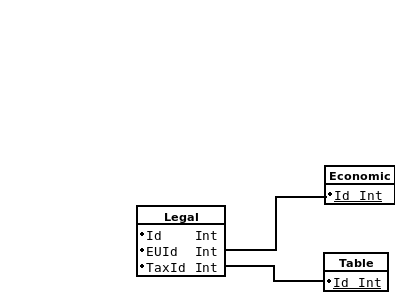
\includegraphics[height=45mm]{fig/units.png}

\item
  \begin{enumerate}
    \item 15 (including the primary and foreign keys).
    \item AlbumId, MediatypeId, GenreId.
    \item Integer
  \end{enumerate}

\item See figure~\ref{fig:ansschema} on page \pageref{fig:ansschema}.
  \begin{figure}[p]
  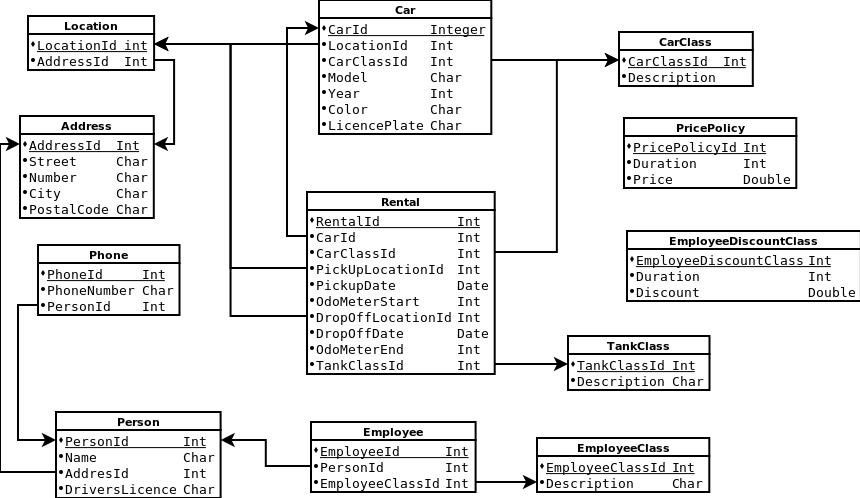
\includegraphics[width=\textwidth]{fig/schema_rentals.png}
  \caption{Car rental ERD.}
  \label{fig:ansschema}
  \end{figure}

\item $\{a,b,c,d,e\}\cap\{b,d,f\}=\{b,d\}$. Furthermore $V\cup W = \{a,b,c,d,e,f\}$,
      $V-W=\{a,c,e\}$, and $W-V=\{f\}$. So $\{a,b,c,d,e,f\}-\{a,c,e\}-\{f\}=\{b,d\}$.
\item 
  \begin{enumerate}
  \item $\Pi_{a\in A}(A\ltimes B) = A$ (note: this is true for any $A$).

  \item 
  $
  \sigma_{Age>40} (A\times B) = \sigma_{Age>40}(A)\times B
  =
  \begin{array}{|lll|}
  \hline
  Name & Age & Height\\
  \hline
  \hline
  \end{array}
  $ (table with zero rows and three columns).
  \item 
  \begin{align*}
  \sigma_{Age\leq40\land Height\leq 170} (A\times B) &= 
    \sigma_{Age\leq 40}(A)\times\sigma_{height\leq 170}(B)\\
  & =
  \begin{array}{|lll|}
  \hline
  Name & Age & Height\\
  \hline
  Mary & 34  & 167\\
  \hline
  \end{array}
  \end{align*}

  \item
  $$
  \Pi_{Height}A\bowtie B 
  = 
  \begin{array}{|l|}
  \hline
   Height\\
  \hline
   178\\
   167\\
  \hline
  \end{array}
  $$
  \end{enumerate}

\item
\begin{enumerate}
\item $\Pi_{Title,Name}(\texttt{tracks}\ltimes_{AlbumId}\texttt{albums})$
\item For readability we define two intermediate results: $X$ and $Y$.
\begin{align*}
X & = \texttt{tracks}\ltimes_{AlbumId}(\texttt{albums}\ltimes_{ArtistId}(\rho_{Name/Artist}\texttt{artists}))\\
Y & = (\texttt{invoice\_items}\ltimes_{TrackId}X)\bowtie\texttt{invoices}\bowtie_{CustomerId}\texttt{customers}\\
& \Pi_{Artist,Name,CustomerId}(Y)
\end{align*}
\item $\Pi_{TrackId,EmployeeId}(Y\bowtie\texttt{employees})$.
\end{enumerate}
\end{enumerate}


%%%%%%%%%%%%%%%%%%%%%%%%%%%%%%%%%%%%%%%%%%%%%%%%%%%%%%%%%%%%%%%%%%%%%%%%%%%%%%%
\section*{Answers for section \ref{sect:exinfomodel}}
\label{sect:ansinfomodel}

\begin{enumerate}
\item
  \begin{enumerate}
  \item One CPU is associated with 0 or more controllers. An SCSI Controller
        is a type of controller. One SCSI controller is associated with 1 to 4
        DiskDrives.
  \item One Bank is associated with 0 or more Accounts. Checking and Saving
        are types of Accounts.
  \end{enumerate}
  \item  See Figure~\ref{fig:ansuml} on page \pageref{fig:ansuml}.
  \begin{figure}[p]
  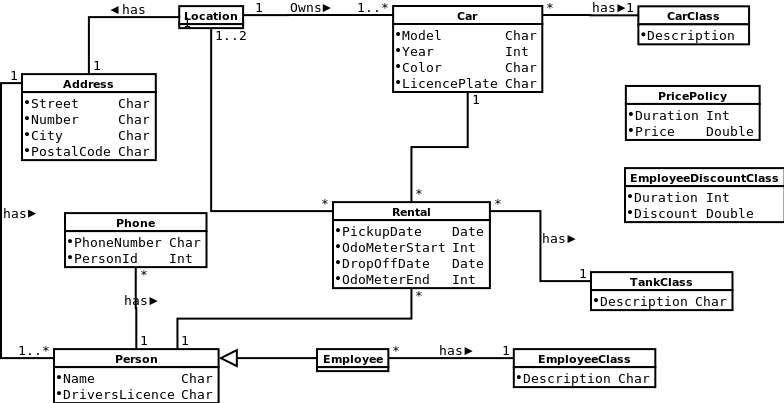
\includegraphics[width=\textwidth]{fig/umldiagram.png}
  \caption{Car rental UML diagram.}
  \label{fig:ansuml}
  \end{figure}
\end{enumerate}


